%! TEX root = ../root/raiz.tex
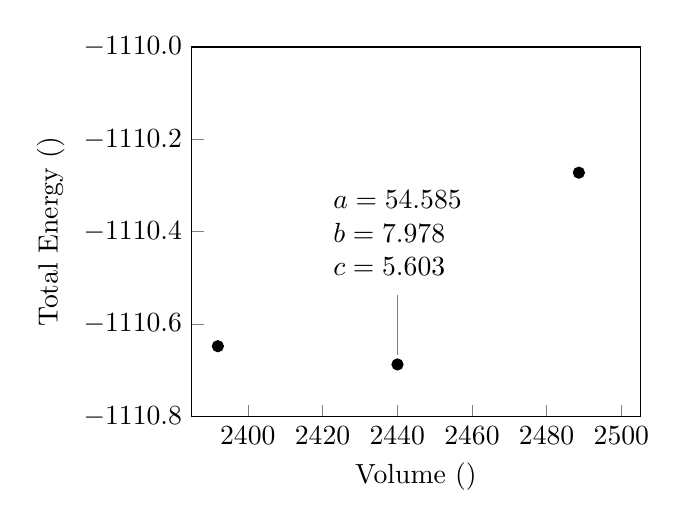
\begin{tikzpicture}
    \begin{axis}
        [
            width=.6\linewidth,
            legend pos={outer north east},
            legend style={draw=none},
            legend cell align=left,
            tick align=inside,
            tick pos=left,
            minor tick num=0,
            xlabel={Volume (\si{\cubic\angstrom})},
            xmin=2385,xmax=2505,
            xticklabel style={
                /pgf/number format/.cd,
                1000 sep={}
            },
            ylabel={Total Energy (\si{\electronvolt})},
            ymin=-1110.8,ymax=-1110,
            yticklabel style={
                /pgf/number format/.cd,
                1000 sep={},
                fixed,
                fixed zerofill,
                precision=1,
                /tikz/.cd
            },
        ]
        \addplot [black, only marks, mark=*] table {
        2391.99 -1110.64777758
        2440.07 -1110.68726343
        2488.62 -1110.27208070
        }
        node [pin={[pin distance=5ex]90:\begin{tabular}{l}$a=\SI{54.585}{\angstrom}$\\$b=\SI{7.978}{\angstrom}$\\$c=\SI{5.603}{\angstrom}$\\\end{tabular}}] at (2440.07, -1110.68726343) {};
    \end{axis}
\end{tikzpicture}
